\documentclass[11pt,a4paper]{report}
\usepackage[utf8]{inputenc}
\usepackage{geometry}
\geometry{margin=1in}
\usepackage{graphicx}
\usepackage{setspace}
\usepackage{titlesec}
\usepackage{array}
\usepackage{booktabs}
\usepackage{caption}
\usepackage{amsmath}
\usepackage{amssymb}
\usepackage{float}
\usepackage{tabularx}
\newcolumntype{Y}{>{\raggedright\arraybackslash}X}
\usepackage{xcolor}
\usepackage{listings}
\usepackage{tikz}
\usetikzlibrary{positioning, shapes.multipart, shapes.geometric, arrows.meta}
\usepackage[hidelinks]{hyperref}

% Section numbering depth
\setcounter{secnumdepth}{3}
\renewcommand{\thesection}{\arabic{section}}

% ------------------ SQL listing style ------------------
\definecolor{codebg}{RGB}{248,248,248}
\definecolor{codekw}{RGB}{0,0,160}
\definecolor{codecm}{RGB}{0,110,0}
\definecolor{codestr}{RGB}{160,0,0}
\lstdefinestyle{sql}{
    language=SQL,
    basicstyle=\ttfamily\scriptsize,
    keywordstyle=\color{codekw}\bfseries,
    commentstyle=\color{codecm}\itshape,
    stringstyle=\color{codestr},
    backgroundcolor=\color{codebg},
    frame=single, rulecolor=\color{gray!60},
    breaklines=true, columns=fullflexible, keepspaces=true,
    showstringspaces=false, tabsize=4,
    numbers=left, numberstyle=\tiny\color{gray}, numbersep=6pt,
    morekeywords={PROCEDURE,FUNCTION,RETURNS,RETURN,LANGUAGE,PLPGSQL,DECLARE,
                  BEGIN,END,IF,ELSIF,THEN,RAISE,EXCEPTION,FOUND,PERFORM,INOUT,
                  RETURNING,FOR,LOOP,SERIAL,FILTER,OVER,RANK,WITH,LIMIT,CALL,
                  COALESCE,GREATEST,LEAST,IMMUTABLE,REPLACE,ROWTYPE,NULLIF,
                  INTERVAL,PARTITION,LATERAL,EXISTS,USING,UNIQUE,INDEX,CHECK}
}
\lstset{style=sql}
\captionsetup[lstlisting]{font=small, labelfont=bf}

% ------------------ Diagram styles ------------------
\tikzset{
  tbl/.style={rectangle split, rectangle split parts=2, draw=blue!50!black,
              rectangle split part fill={blue!15,white}, font=\scriptsize,
              text width=2.75cm, align=left, inner sep=2.5pt, anchor=north},
  fk/.style={-{Stealth[length=2mm]}, thick, gray!40!black},
  st/.style={draw, rounded corners=3pt, fill=green!8, font=\footnotesize\ttfamily,
             minimum width=2.2cm, minimum height=0.8cm, align=center},
  tr/.style={-{Stealth[length=2mm]}, thick},
  lbl/.style={font=\scriptsize, align=center}
}

\begin{document}

% ------------------ Cover Page ------------------

\begin{titlepage}
    \centering

    % Ensure 'College Logo RGB.jpg' is in your project folder.
    
\includegraphics[width=5cm]{College Logo RGB.jpg}\\[1cm]

    \vspace{1cm}
    \textbf{\large A Case Study on} \\[0.5cm]
    {\LARGE \textbf{Database Design for a Library Management System}}\\[0.4cm]
    {\large \textbf{Resource Tracking, Lending Operations, and Fine Administration}}\\[1.5cm]

    {\Large A9511 - Database Management Systems}\\[1.5cm]

    \textbf{Submitted by}\\ [0.25cm]
    Batch No. 6

    \begin{center}
        \begin{table}[h!]
            \centering
            \setstretch{1.2}
            \begin{tabular}{l l}
                {Madhavarapu Saritha} & {25881A05V7}\\ [2mm]
                {Chepyala Vishal} & {25881A05X9}\\ [2mm]
                {Gundu Srijay Krishna} & {25881A05X0}\\ [2mm]
            \end{tabular}
        \end{table}
    \end{center}

    \vspace{0.5cm}
    \textbf{Course Facilitator}\\ [0.1in]
    {Dr. Reddy Saisindhutheja}\\
    Associate Professor\\[2.5cm]

    {\large\textbf{Department of Computer Science and Engineering}}\\[0.5cm]
    {\large\textbf{Vardhaman College of Engineering, Hyderabad}}\\[0.5cm]
    {\large \textbf{November 2026}}

\end{titlepage}

% ------------------ Contents ------------------

\tableofcontents
\newpage

% ------------------ Section 1: Problem Definition ------------------

\section{Problem Definition and Context}

\subsection{Library Management as a Database Problem}
A college library lends thousands of books every semester to students, faculty and staff. Many libraries still keep this information in paper registers or loosely structured spreadsheets. As a result, it is difficult to answer simple questions such as \emph{``Is a copy of this book on the shelf?''}, \emph{``Who has had this copy for more than two weeks?''} or \emph{``How much does this member owe?''}. Errors in these records lead to lost books, disputes over fines and unfair treatment of members waiting for popular titles.

\textbf{Problem Statement:} Model books, copies, members, issue/return records, fines and reservations. Build the schema, stored procedures for issuing and returning books, and queries for overdue books, popular titles and member-wise fines.

The case study analyses four questions:
\begin{itemize}
    \item \textbf{Title vs.\ copy:} the difference between a book title and its physical copies, and how members, issues and returns relate.
    \item \textbf{Issue rules:} borrowing limits, due dates and the fine calculation logic.
    \item \textbf{Reservations:} how requests are handled when all copies of a title are issued.
    \item \textbf{Reporting:} overdue, popular-title and member-wise fine queries.
\end{itemize}

The solution is implemented and tested on \textbf{PostgreSQL 16} using PL/pgSQL stored procedures. Every output in this report was produced by actually running the scripts on the sample data described in Section~\ref{sec:testing}.

\subsection{Relevance to Sustainable Development Goals (SDGs)}
A well-designed library database supports the following UN SDGs:
\begin{itemize}
    \item \textbf{SDG 4 (Quality Education):} Reliable, quick access to textbooks and reference material supports Target 4.3 (equal access to quality tertiary education).
    \item \textbf{SDG 10 (Reduced Inequalities):} A first-come-first-served reservation queue and capped fines make sure students who cannot afford their own textbooks get fair access to shared copies.
    \item \textbf{SDG 12 (Responsible Consumption and Production):} Sharing and reusing physical copies, and buying new copies only where demand data justifies it, reduces paper and resource waste (Target 12.5).
\end{itemize}

% ------------------ Section 2: Problem Analysis ------------------

\section{Problem Analysis and Solution Development}

\subsection{Characterization of the Problem}
At first glance a library looks like a simple ``books and borrowers'' application. In practice, however, the database has to enforce several rules that interact with each other:
\begin{itemize}
    \item A \emph{title} (e.g.\ \textit{Database System Concepts}, 7th ed.) has many \emph{physical copies}. Members borrow copies, but they search for and reserve titles.
    \item Borrowing limits, loan periods and fine rates depend on the member category (student, faculty, staff).
    \item A copy that is returned while other members are waiting must go to the \emph{right} person in the queue, not back to the open shelf.
    \item Two librarians working at two counters must never lend the same copy twice, or let a member exceed their limit by issuing at the same moment.
\end{itemize}
These rules belong \emph{inside} the database, as constraints and stored procedures, so that no front-end program can bypass them.

\subsection{Engineering Knowledge Applied}
\begin{itemize}
    \item \textbf{Conceptual Modelling:} Entity--Relationship (ER) modelling with cardinality and participation constraints.
    \item \textbf{Normalization:} Functional-dependency analysis to bring every relation to Third Normal Form (3NF)/BCNF.
    \item \textbf{Integrity Constraints:} Primary/foreign keys, \texttt{CHECK} constraints and \emph{partial unique indexes} that encode business rules declaratively.
    \item \textbf{Procedural SQL:} PL/pgSQL stored procedures for issue, return, reservation, hold expiry and fine payment.
    \item \textbf{Transactions and Concurrency Control:} Row-level locks (\texttt{SELECT \dots\ FOR UPDATE}) and a fixed lock order to prevent double issue and deadlocks.
    \item \textbf{Analytical SQL:} Joins, aggregation with \texttt{FILTER}, Common Table Expressions (CTEs) and window functions (\texttt{RANK()}).
\end{itemize}

\subsection{Title vs.\ Physical Copy and How Members, Issues and Returns Relate}
\label{sec:er}
The central design decision is to keep the \textbf{bibliographic title} (\texttt{book}) separate from the \textbf{physical item} (\texttt{book\_copy}):
\begin{itemize}
    \item \texttt{book} holds what is common to every copy: ISBN, title, edition, publisher, year. A title is described once, no matter how many copies the library buys.
    \item \texttt{book\_copy} holds what differs between copies: a unique barcode, shelf location, acquisition date and the \emph{current status} (\texttt{AVAILABLE}, \texttt{ISSUED}, \texttt{ON\_HOLD}, \texttt{LOST}, \texttt{DAMAGED}).
    \item A \texttt{loan} links one \emph{copy} to one \emph{member} for a period of time. The issue is the \texttt{INSERT}; the return is the \texttt{UPDATE} that fills \texttt{return\_date}. One row therefore records the whole issue/return cycle.
    \item A \texttt{reservation} is placed on a \emph{title}, not on a copy: a member wants ``any copy of \textit{Clean Code}'', whichever is returned first.
    \item A \texttt{fine} is generated by at most one loan, so \texttt{fine.loan\_id} is \texttt{UNIQUE}.
\end{itemize}

Figure~\ref{fig:er} shows the resulting relational schema. Arrows point from a foreign key to the referenced (parent) table.

\begin{figure}[H]
\centering
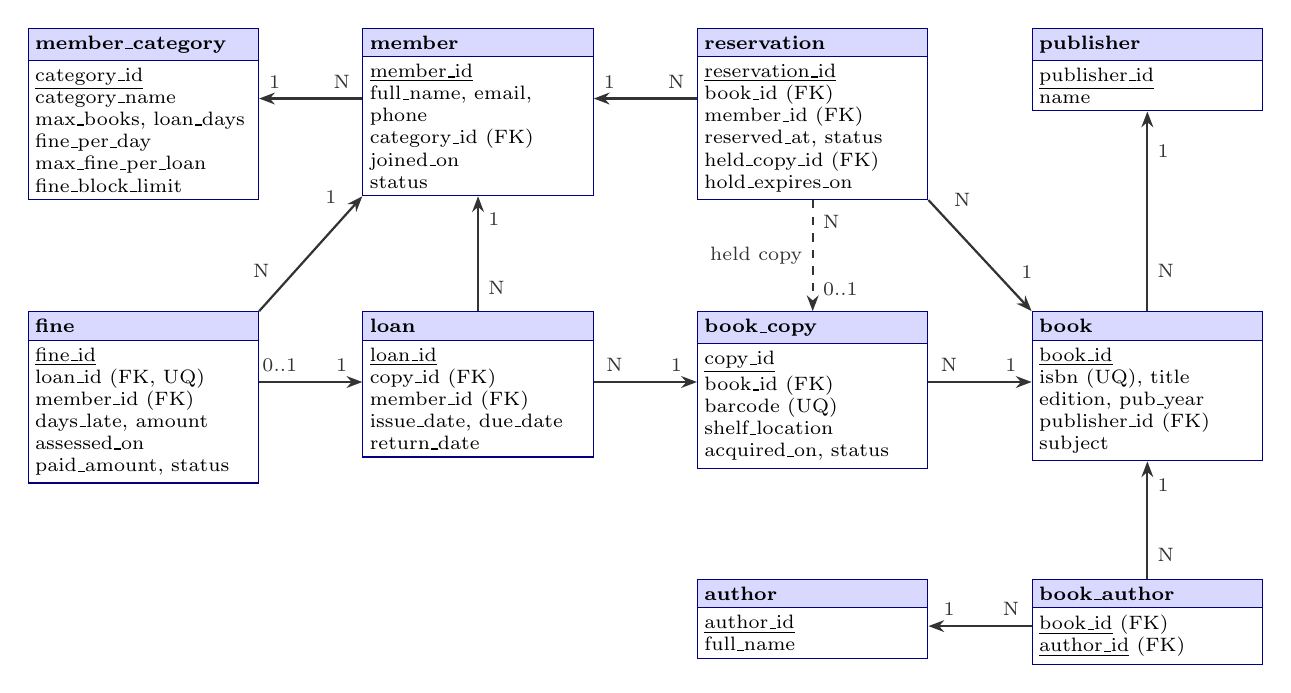
\begin{tikzpicture}[node distance=1cm]
  % Row A
  \node[tbl] (cat) at (0,0) {\textbf{member\_category}\nodepart{two}\underline{category\_id}\\category\_name\\max\_books, loan\_days\\fine\_per\_day\\max\_fine\_per\_loan\\fine\_block\_limit};
  \node[tbl] (mem) at (4.25,0) {\textbf{member}\nodepart{two}\underline{member\_id}\\full\_name, email, phone\\category\_id (FK)\\joined\_on\\status};
  \node[tbl] (res) at (8.5,0) {\textbf{reservation}\nodepart{two}\underline{reservation\_id}\\book\_id (FK)\\member\_id (FK)\\reserved\_at, status\\held\_copy\_id (FK)\\hold\_expires\_on};
  \node[tbl] (pub) at (12.75,0) {\textbf{publisher}\nodepart{two}\underline{publisher\_id}\\name};
  % Row B
  \node[tbl] (fine) at (0,-3.6) {\textbf{fine}\nodepart{two}\underline{fine\_id}\\loan\_id (FK, UQ)\\member\_id (FK)\\days\_late, amount\\assessed\_on\\paid\_amount, status};
  \node[tbl] (loan) at (4.25,-3.6) {\textbf{loan}\nodepart{two}\underline{loan\_id}\\copy\_id (FK)\\member\_id (FK)\\issue\_date, due\_date\\return\_date};
  \node[tbl] (copy) at (8.5,-3.6) {\textbf{book\_copy}\nodepart{two}\underline{copy\_id}\\book\_id (FK)\\barcode (UQ)\\shelf\_location\\acquired\_on, status};
  \node[tbl] (book) at (12.75,-3.6) {\textbf{book}\nodepart{two}\underline{book\_id}\\isbn (UQ), title\\edition, pub\_year\\publisher\_id (FK)\\subject};
  % Row C
  \node[tbl] (auth) at (8.5,-7.0) {\textbf{author}\nodepart{two}\underline{author\_id}\\full\_name};
  \node[tbl] (ba) at (12.75,-7.0) {\textbf{book\_author}\nodepart{two}\underline{book\_id} (FK)\\\underline{author\_id} (FK)};
  % Relationships (child -> parent)
  \draw[fk] (mem.west |- 0,-0.9) -- node[lbl,above,pos=0.2]{N} node[lbl,above,pos=0.85]{1} (cat.east |- 0,-0.9);
  \draw[fk] (res.west |- 0,-0.9) -- node[lbl,above,pos=0.2]{N} node[lbl,above,pos=0.85]{1} (mem.east |- 0,-0.9);
  \draw[fk] (loan.north) -- node[lbl,right,pos=0.2]{N} node[lbl,right,pos=0.8]{1} (mem.south);
  \draw[fk] (fine.east |- 0,-4.5) -- node[lbl,above,pos=0.2]{0..1} node[lbl,above,pos=0.8]{1} (loan.west |- 0,-4.5);
  \draw[fk] (fine.north east) -- node[lbl,above left,pos=0.2]{N} node[lbl,above left,pos=0.85]{1} (mem.south west);
  \draw[fk] (loan.east |- 0,-4.5) -- node[lbl,above,pos=0.2]{N} node[lbl,above,pos=0.8]{1} (copy.west |- 0,-4.5);
  \draw[fk] (copy.east |- 0,-4.5) -- node[lbl,above,pos=0.2]{N} node[lbl,above,pos=0.8]{1} (book.west |- 0,-4.5);
  \draw[fk] (res.south east) -- node[lbl,above right,pos=0.15]{N} node[lbl,above right,pos=0.8]{1} (book.north west);
  \draw[fk, dashed] (res.south) -- node[lbl,right,pos=0.2]{N} node[lbl,right,pos=0.8]{0..1} node[lbl,left,pos=0.5]{held copy} (copy.north);
  \draw[fk] (book.north) -- node[lbl,right,pos=0.2]{N} node[lbl,right,pos=0.8]{1} (pub.south);
  \draw[fk] (ba.north) -- node[lbl,right,pos=0.2]{N} node[lbl,right,pos=0.8]{1} (book.south);
  \draw[fk] (ba.west |- 0,-7.6) -- node[lbl,above,pos=0.2]{N} node[lbl,above,pos=0.8]{1} (auth.east |- 0,-7.6);
\end{tikzpicture}
\caption{Relational schema of the Library Management System (PK underlined, FK = foreign key, UQ = unique)}
\label{fig:er}
\end{figure}

\subsubsection{Normalization}
The main functional dependencies (FDs) are:
\begin{align*}
\texttt{isbn} &\rightarrow \texttt{title, edition, publisher\_id, pub\_year, subject}\\
\texttt{barcode} &\rightarrow \texttt{copy\_id, book\_id, shelf\_location, acquired\_on, status}\\
\texttt{category\_id} &\rightarrow \texttt{max\_books, loan\_days, fine\_per\_day, \dots}\\
\texttt{loan\_id} &\rightarrow \texttt{copy\_id, member\_id, issue\_date, due\_date, return\_date}
\end{align*}
If title data were stored in every copy row, the FD $\texttt{isbn} \rightarrow \texttt{title}$ would be a transitive dependency ($\texttt{copy\_id} \rightarrow \texttt{isbn} \rightarrow \texttt{title}$), which violates 3NF and causes update anomalies (changing a title in one copy but not another). Likewise, storing \texttt{max\_books} in \texttt{member} would repeat the rule for every student. Splitting into \texttt{book}/\texttt{book\_copy} and \texttt{member}/\texttt{member\_category} leaves every non-key attribute depending only on its table's key. Authors are many-to-many with books, so they are resolved through \texttt{book\_author}. Every relation is therefore in \textbf{BCNF}.

\subsubsection{Schema Highlights}
Listing~\ref{lst:schema} shows the core tables. Two partial unique indexes encode business rules that a plain \texttt{UNIQUE} constraint cannot express:
\begin{itemize}
    \item \texttt{uq\_loan\_open\_copy}: a copy can be on \emph{at most one open loan} (one with \texttt{return\_date IS NULL}), while any number of closed loans are allowed as history.
    \item \texttt{uq\_resv\_live}: a member may hold only one \emph{live} (\texttt{WAITING}/\texttt{READY}) reservation per title.
\end{itemize}

\begin{lstlisting}[caption={Core tables and constraints (from \texttt{01\_schema.sql})}, label={lst:schema}]
CREATE TABLE book (                       -- one row per TITLE / edition
    book_id      SERIAL       PRIMARY KEY,
    isbn         CHAR(13)     NOT NULL UNIQUE,
    title        VARCHAR(200) NOT NULL,
    edition      SMALLINT     NOT NULL DEFAULT 1,
    publisher_id INT          REFERENCES publisher,
    pub_year     SMALLINT     CHECK (pub_year BETWEEN 1800 AND 2100),
    subject      VARCHAR(60)
);
CREATE TABLE book_copy (                  -- one row per PHYSICAL item
    copy_id        SERIAL      PRIMARY KEY,
    book_id        INT         NOT NULL REFERENCES book,
    barcode        VARCHAR(20) NOT NULL UNIQUE,
    shelf_location VARCHAR(20),
    acquired_on    DATE        NOT NULL DEFAULT CURRENT_DATE,
    status         VARCHAR(10) NOT NULL DEFAULT 'AVAILABLE'
                   CHECK (status IN ('AVAILABLE','ISSUED','ON_HOLD','LOST','DAMAGED'))
);
CREATE TABLE loan (
    loan_id     SERIAL  PRIMARY KEY,
    copy_id     INT     NOT NULL REFERENCES book_copy,
    member_id   INT     NOT NULL REFERENCES member,
    issue_date  DATE    NOT NULL DEFAULT CURRENT_DATE,
    due_date    DATE    NOT NULL,
    return_date DATE,
    CHECK (due_date > issue_date),
    CHECK (return_date IS NULL OR return_date >= issue_date)
);
-- A copy can be on at most ONE open loan at any time
CREATE UNIQUE INDEX uq_loan_open_copy ON loan (copy_id) WHERE return_date IS NULL;

CREATE TABLE reservation (                -- placed on a TITLE, not a copy
    reservation_id  SERIAL      PRIMARY KEY,
    book_id         INT         NOT NULL REFERENCES book,
    member_id       INT         NOT NULL REFERENCES member,
    reserved_at     TIMESTAMP   NOT NULL DEFAULT now(),
    status          VARCHAR(10) NOT NULL DEFAULT 'WAITING'
                    CHECK (status IN ('WAITING','READY','FULFILLED','CANCELLED','EXPIRED')),
    held_copy_id    INT         REFERENCES book_copy,
    hold_expires_on DATE,
    CHECK (status <> 'READY'   OR (held_copy_id IS NOT NULL AND hold_expires_on IS NOT NULL)),
    CHECK (status <> 'WAITING' OR held_copy_id IS NULL)
);
CREATE UNIQUE INDEX uq_resv_live ON reservation (book_id, member_id)
    WHERE status IN ('WAITING','READY');

CREATE TABLE fine (                       -- at most one fine per loan
    fine_id     SERIAL       PRIMARY KEY,
    loan_id     INT          NOT NULL UNIQUE REFERENCES loan,
    member_id   INT          NOT NULL REFERENCES member,
    days_late   INT          NOT NULL CHECK (days_late > 0),
    amount      NUMERIC(8,2) NOT NULL CHECK (amount >= 0),
    assessed_on DATE         NOT NULL DEFAULT CURRENT_DATE,
    paid_amount NUMERIC(8,2) NOT NULL DEFAULT 0 CHECK (paid_amount >= 0),
    status      VARCHAR(8)   NOT NULL DEFAULT 'UNPAID'
                CHECK (status IN ('UNPAID','PAID','WAIVED')),
    CHECK (paid_amount <= amount)
);
\end{lstlisting}

A view \texttt{v\_title\_availability} combines both levels for the circulation desk. Table~\ref{tab:avail} shows its output for the sample data: the library holds 8 titles but 13 physical copies.

\begin{table}[H]
    \centering
    \caption{Title-level availability computed from copy-level status (before the test run)}
    \label{tab:avail}
    \footnotesize
    \begin{tabular}{|l|c|c|c|c|c|}
        \hline
        \textbf{Title} & \textbf{Copies} & \textbf{Available} & \textbf{Issued} & \textbf{On hold} & \textbf{Queue} \\ \hline
        Database System Concepts & 3 & 1 & 2 & 0 & 0 \\ \hline
        Fundamentals of Database Systems & 2 & 1 & 1 & 0 & 0 \\ \hline
        Introduction to Algorithms & 2 & 1 & 1 & 0 & 0 \\ \hline
        Operating System Concepts & 2 & 1 & 1 & 0 & 0 \\ \hline
        Computer Networks & 1 & 0 & 1 & 0 & 1 \\ \hline
        Clean Code & 1 & 0 & 1 & 0 & 2 \\ \hline
        The Pragmatic Programmer & 1 & 1 & 0 & 0 & 0 \\ \hline
        Design Patterns & 1 & 1 & 0 & 0 & 0 \\ \hline
    \end{tabular}
\end{table}

\subsection{Issue Rules and Fine Calculation Logic}
\label{sec:rules}
\subsubsection{Borrowing Rules}
Rules are stored as \emph{data} in \texttt{member\_category}, not hard-coded, so the library committee can change them without touching any program (Table~\ref{tab:rules}).

\begin{table}[H]
    \centering
    \caption{Borrowing rules per member category}
    \label{tab:rules}
    \small
    \setstretch{1.2}
    \begin{tabular}{|l|c|c|c|c|c|}
        \hline
        \textbf{Category} & \textbf{Max books} & \textbf{Loan days} & \textbf{Fine/day} & \textbf{Cap per loan} & \textbf{Block if unpaid $>$} \\ \hline
        Student & 3 & 14 & Rs.\,2 & Rs.\,200 & Rs.\,100 \\ \hline
        Faculty & 8 & 30 & Rs.\,1 & Rs.\,100 & Rs.\,200 \\ \hline
        Staff   & 4 & 21 & Rs.\,1 & Rs.\,100 & Rs.\,100 \\ \hline
    \end{tabular}
\end{table}

\subsubsection{Mathematical Formulation}
Let member $m$ belong to category $c$ with borrowing limit $L_c$, loan period $T_c$, daily fine rate $r_c$, fine cap $F^{\max}_c$ and blocking limit $B_c$.

\textbf{Eligibility to borrow.} With $n_m$ = number of open loans, $o_m$ = number of overdue open loans and $U_m$ = total unpaid fines,
$$\text{Eligible}(m) \iff s_m = \texttt{ACTIVE} \;\wedge\; o_m = 0 \;\wedge\; n_m < L_c \;\wedge\; U_m \le B_c$$

\textbf{Due date.} For a copy issued on date $d_i$:
$$d_{due} = d_i + T_c$$

\textbf{Fine.} When the copy is returned on date $d_r$:
$$F = \min\Big(r_c \cdot \max\big(0,\; d_r - d_{due}\big),\; F^{\max}_c\Big)$$

\textit{Worked example:} a student returns a book 26 days late, so $F = \min(2 \times 26,\; 200) = \text{Rs.\,}52$. If the same book were 120 days late, $F = \min(240, 200) = \text{Rs.\,}200$. The cap keeps a forgotten book from turning into an unaffordable debt.

\textbf{Expected wait for a reservation.} If a title has $n$ copies, all issued, and a member is at position $k$ in the queue, then in the worst case the member waits for
$$W_k \le \left\lceil \frac{k}{n} \right\rceil \cdot T_c \;+\; \left(\left\lceil \frac{k}{n} \right\rceil - 1\right)\cdot H$$
days, where $H = 3$ days is the pick-up window given to each earlier member in the queue.

\subsubsection{Fine Function and Issue Procedure}
\begin{lstlisting}[caption={Fine calculation and the \texttt{sp\_issue\_book} procedure}, label={lst:issue}]
CREATE OR REPLACE FUNCTION fn_calculate_fine(p_due DATE, p_returned DATE,
                                             p_rate NUMERIC, p_cap NUMERIC)
RETURNS NUMERIC LANGUAGE sql IMMUTABLE AS $$
    SELECT LEAST(GREATEST(p_returned - p_due, 0) * p_rate, p_cap)::NUMERIC(8,2);
$$;

CREATE OR REPLACE PROCEDURE sp_issue_book(p_member_id INT, p_barcode VARCHAR,
                                          INOUT p_loan_id INT  DEFAULT NULL,
                                          INOUT p_due_date DATE DEFAULT NULL)
LANGUAGE plpgsql AS $$
DECLARE
    v_mem     RECORD;
    v_copy    book_copy%ROWTYPE;
    v_active  INT;
    v_overdue INT;
    v_unpaid  NUMERIC;
BEGIN
    -- 1. Lock the member: two parallel issues cannot both pass the limit check
    SELECT m.status, c.max_books, c.loan_days, c.fine_block_limit INTO v_mem
      FROM member m JOIN member_category c USING (category_id)
     WHERE m.member_id = p_member_id
       FOR UPDATE OF m;
    IF NOT FOUND THEN
        RAISE EXCEPTION 'Member % does not exist', p_member_id;
    END IF;
    IF v_mem.status <> 'ACTIVE' THEN
        RAISE EXCEPTION 'Member % is %', p_member_id, v_mem.status;
    END IF;

    -- 2. Borrowing rules
    SELECT COUNT(*), COUNT(*) FILTER (WHERE due_date < CURRENT_DATE)
      INTO v_active, v_overdue
      FROM loan
     WHERE member_id = p_member_id AND return_date IS NULL;

    IF v_overdue > 0 THEN
        RAISE EXCEPTION 'Member % has % overdue book(s); return them first',
                        p_member_id, v_overdue;
    END IF;
    IF v_active >= v_mem.max_books THEN
        RAISE EXCEPTION 'Borrowing limit reached: % of % books already issued',
                        v_active, v_mem.max_books;
    END IF;

    SELECT COALESCE(SUM(amount - paid_amount), 0) INTO v_unpaid
      FROM fine WHERE member_id = p_member_id AND status = 'UNPAID';
    IF v_unpaid > v_mem.fine_block_limit THEN
        RAISE EXCEPTION 'Unpaid fines Rs.% exceed the limit of Rs.%',
                        v_unpaid, v_mem.fine_block_limit;
    END IF;

    -- 3. Lock the copy and make sure it may be lent to THIS member
    SELECT * INTO v_copy FROM book_copy WHERE barcode = p_barcode FOR UPDATE;
    IF NOT FOUND THEN
        RAISE EXCEPTION 'No copy with barcode %', p_barcode;
    END IF;

    IF v_copy.status = 'ON_HOLD' THEN
        UPDATE reservation SET status = 'FULFILLED'
         WHERE held_copy_id = v_copy.copy_id AND status = 'READY'
           AND member_id = p_member_id;
        IF NOT FOUND THEN
            RAISE EXCEPTION 'Copy % is on hold for another member', p_barcode;
        END IF;
    ELSIF v_copy.status <> 'AVAILABLE' THEN
        RAISE EXCEPTION 'Copy % is not available (status %)', p_barcode, v_copy.status;
    END IF;

    IF EXISTS (SELECT 1 FROM loan l JOIN book_copy c USING (copy_id)
                WHERE l.member_id = p_member_id AND l.return_date IS NULL
                  AND c.book_id = v_copy.book_id) THEN
        RAISE EXCEPTION 'Member % already has a copy of this title', p_member_id;
    END IF;

    -- 4. Record the loan
    p_due_date := CURRENT_DATE + v_mem.loan_days;
    INSERT INTO loan (copy_id, member_id, issue_date, due_date)
    VALUES (v_copy.copy_id, p_member_id, CURRENT_DATE, p_due_date)
    RETURNING loan_id INTO p_loan_id;

    UPDATE book_copy SET status = 'ISSUED' WHERE copy_id = v_copy.copy_id;
END $$;
\end{lstlisting}

\subsubsection{Return Procedure}
Returning a copy closes the loan, assesses the fine with the formula above and then hands the copy to the reservation queue (Section~\ref{sec:resv}).

\begin{lstlisting}[caption={The \texttt{sp\_return\_book} procedure}, label={lst:return}]
CREATE OR REPLACE PROCEDURE sp_return_book(p_barcode VARCHAR,
                                           p_return_date DATE DEFAULT CURRENT_DATE,
                                           INOUT p_fine NUMERIC DEFAULT 0,
                                           INOUT p_held_for INT DEFAULT NULL)
LANGUAGE plpgsql AS $$
DECLARE
    v_loan loan%ROWTYPE;
    v_rate NUMERIC;
    v_cap  NUMERIC;
BEGIN
    SELECT l.* INTO v_loan
      FROM loan l JOIN book_copy c USING (copy_id)
     WHERE c.barcode = p_barcode AND l.return_date IS NULL
       FOR UPDATE OF l, c;
    IF NOT FOUND THEN
        RAISE EXCEPTION 'Copy % is not currently on loan', p_barcode;
    END IF;
    IF p_return_date < v_loan.issue_date OR p_return_date > CURRENT_DATE THEN
        RAISE EXCEPTION 'Invalid return date %', p_return_date;
    END IF;

    UPDATE loan SET return_date = p_return_date WHERE loan_id = v_loan.loan_id;

    -- Fine assessment
    SELECT mc.fine_per_day, mc.max_fine_per_loan INTO v_rate, v_cap
      FROM member m JOIN member_category mc USING (category_id)
     WHERE m.member_id = v_loan.member_id;

    p_fine := fn_calculate_fine(v_loan.due_date, p_return_date, v_rate, v_cap);
    IF p_fine > 0 THEN
        INSERT INTO fine (loan_id, member_id, days_late, amount, assessed_on)
        VALUES (v_loan.loan_id, v_loan.member_id,
                p_return_date - v_loan.due_date, p_fine, p_return_date);
    END IF;

    -- Hand the copy to the reservation queue (or back to the shelf)
    p_held_for := fn_allocate_copy(v_loan.copy_id);
END $$;
\end{lstlisting}

A separate procedure \texttt{sp\_pay\_fine(fine\_id, amount)} records full or part payments. It marks the fine \texttt{PAID} only when the balance reaches zero and rejects over-payment.

\subsection{Handling of Reservations When All Copies Are Issued}
\label{sec:resv}
A reservation is accepted \emph{only} when no copy of the title is on the shelf; otherwise the member is told to borrow the available copy. Reservations form a \textbf{FIFO queue per title}, ordered by \texttt{reserved\_at}. Figure~\ref{fig:states} shows how the status of a copy and of a reservation change together.

\begin{figure}[H]
\centering
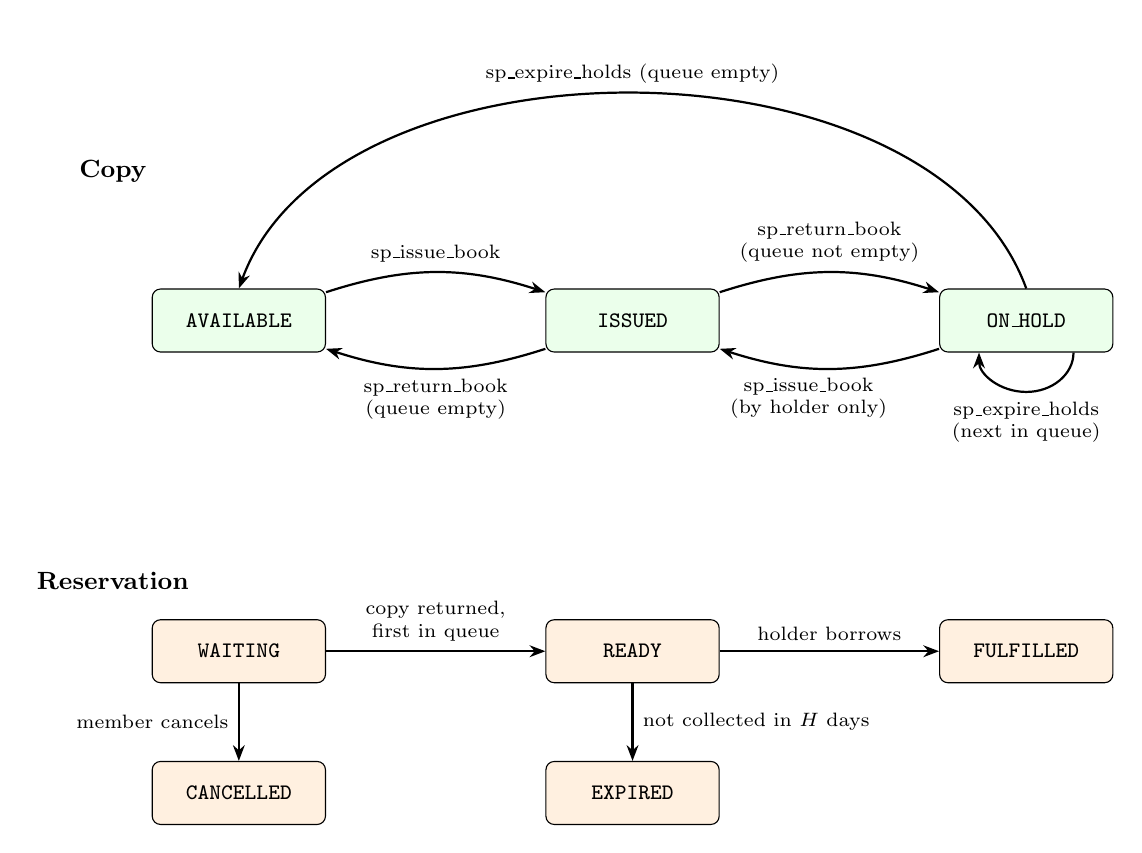
\begin{tikzpicture}
  % Copy life-cycle
  \node[st] (av) at (0,0) {AVAILABLE};
  \node[st] (is) at (5,0) {ISSUED};
  \node[st] (oh) at (10,0) {ON\_HOLD};
  \draw[tr] (av) to[bend left=18] node[lbl,above]{sp\_issue\_book} (is);
  \draw[tr] (is) to[bend left=18] node[lbl,below]{sp\_return\_book\\(queue empty)} (av);
  \draw[tr] (is) to[bend left=18] node[lbl,above]{sp\_return\_book\\(queue not empty)} (oh);
  \draw[tr] (oh) to[bend left=18] node[lbl,below,pos=0.6]{sp\_issue\_book\\(by holder only)} (is);
  \draw[tr] (oh.north) to[out=110,in=70,looseness=0.9] node[lbl,above]{sp\_expire\_holds (queue empty)} (av.north);
  \draw[tr] ([xshift=6mm]oh.south) arc[start angle=0, end angle=-180, x radius=6mm, y radius=5mm] node[lbl,below=5mm,xshift=6mm]{sp\_expire\_holds\\(next in queue)};
  \node[font=\small\bfseries] at (-1.6,1.9) {Copy};
  % Reservation life-cycle
  \node[st, fill=orange!12] (wa) at (0,-4.2) {WAITING};
  \node[st, fill=orange!12] (re) at (5,-4.2) {READY};
  \node[st, fill=orange!12] (fu) at (10,-4.2) {FULFILLED};
  \node[st, fill=orange!12] (ex) at (5,-6.0) {EXPIRED};
  \node[st, fill=orange!12] (ca) at (0,-6.0) {CANCELLED};
  \draw[tr] (wa) -- node[lbl,above]{copy returned,\\first in queue} (re);
  \draw[tr] (re) -- node[lbl,above]{holder borrows} (fu);
  \draw[tr] (re) -- node[lbl,right]{not collected in $H$ days} (ex);
  \draw[tr] (wa) -- node[lbl,left]{member cancels} (ca);
  \node[font=\small\bfseries] at (-1.6,-3.3) {Reservation};
\end{tikzpicture}
\caption{State transitions of a physical copy and of a reservation}
\label{fig:states}
\end{figure}

The queue logic lives in one function, \texttt{fn\_allocate\_copy}, which is used by the return procedure, by the nightly hold-expiry job and when new copies are added:

\begin{lstlisting}[caption={Queue allocation and reservation procedures}, label={lst:resv}]
CREATE OR REPLACE FUNCTION fn_allocate_copy(p_copy_id INT)
RETURNS INT LANGUAGE plpgsql AS $$
DECLARE
    v_book_id INT;
    v_resv    RECORD;
BEGIN
    SELECT book_id INTO v_book_id FROM book_copy WHERE copy_id = p_copy_id FOR UPDATE;
    -- Lock the title so a concurrent sp_reserve_book cannot slip in between
    PERFORM 1 FROM book WHERE book_id = v_book_id FOR UPDATE;

    SELECT reservation_id, member_id INTO v_resv
      FROM reservation
     WHERE book_id = v_book_id AND status = 'WAITING'
     ORDER BY reserved_at, reservation_id
     LIMIT 1
       FOR UPDATE;

    IF FOUND THEN
        UPDATE reservation
           SET status = 'READY', held_copy_id = p_copy_id,
               hold_expires_on = CURRENT_DATE + 3          -- 3-day pickup window
         WHERE reservation_id = v_resv.reservation_id;
        UPDATE book_copy SET status = 'ON_HOLD' WHERE copy_id = p_copy_id;
        RETURN v_resv.member_id;
    END IF;

    UPDATE book_copy SET status = 'AVAILABLE' WHERE copy_id = p_copy_id;
    RETURN NULL;
END $$;

CREATE OR REPLACE PROCEDURE sp_reserve_book(p_member_id INT, p_book_id INT,
                                            INOUT p_reservation_id INT DEFAULT NULL,
                                            INOUT p_queue_position INT DEFAULT NULL)
LANGUAGE plpgsql AS $$
DECLARE
    v_status VARCHAR;
BEGIN
    SELECT status INTO v_status FROM member WHERE member_id = p_member_id;
    IF NOT FOUND OR v_status <> 'ACTIVE' THEN
        RAISE EXCEPTION 'Member % cannot place reservations', p_member_id;
    END IF;

    -- Serialise against fn_allocate_copy for the same title
    PERFORM 1 FROM book WHERE book_id = p_book_id FOR UPDATE;
    IF NOT FOUND THEN
        RAISE EXCEPTION 'Book % does not exist', p_book_id;
    END IF;

    IF EXISTS (SELECT 1 FROM book_copy
                WHERE book_id = p_book_id AND status = 'AVAILABLE') THEN
        RAISE EXCEPTION 'A copy is on the shelf - issue it instead of reserving';
    END IF;
    IF EXISTS (SELECT 1 FROM loan l JOIN book_copy c USING (copy_id)
                WHERE c.book_id = p_book_id AND l.member_id = p_member_id
                  AND l.return_date IS NULL) THEN
        RAISE EXCEPTION 'Member % already has this title on loan', p_member_id;
    END IF;

    BEGIN
        INSERT INTO reservation (book_id, member_id)
        VALUES (p_book_id, p_member_id)
        RETURNING reservation_id INTO p_reservation_id;
    EXCEPTION WHEN unique_violation THEN
        RAISE EXCEPTION 'Member % already has a live reservation for book %',
                        p_member_id, p_book_id;
    END;

    SELECT COUNT(*) INTO p_queue_position
      FROM reservation
     WHERE book_id = p_book_id AND status = 'WAITING'
       AND reservation_id <= p_reservation_id;
END $$;

-- Nightly job: expire holds not collected in time, pass copy onward
CREATE OR REPLACE PROCEDURE sp_expire_holds(INOUT p_expired INT DEFAULT 0)
LANGUAGE plpgsql AS $$
DECLARE
    r RECORD;
BEGIN
    p_expired := 0;
    FOR r IN SELECT reservation_id, held_copy_id FROM reservation
              WHERE status = 'READY' AND hold_expires_on < CURRENT_DATE
    LOOP
        -- lock order copy -> reservation, same as sp_issue_book (no deadlock)
        PERFORM 1 FROM book_copy WHERE copy_id = r.held_copy_id FOR UPDATE;
        UPDATE reservation SET status = 'EXPIRED'
         WHERE reservation_id = r.reservation_id AND status = 'READY';
        IF FOUND THEN
            PERFORM fn_allocate_copy(r.held_copy_id);
            p_expired := p_expired + 1;
        END IF;
    END LOOP;
END $$;
\end{lstlisting}

\subsubsection{Concurrency Analysis}
Two dangerous race conditions were identified and closed:
\begin{enumerate}
    \item \textbf{Double issue / limit overrun.} Two counters issuing to the same member at the same moment could both read ``2 of 3 books'' and both succeed. \texttt{sp\_issue\_book} therefore locks the member row first (\texttt{FOR UPDATE OF m}), so the second transaction waits and then sees 3 open loans. The partial unique index \texttt{uq\_loan\_open\_copy} is a second line of defence: even a buggy program cannot open two loans on one copy.
    \item \textbf{Lost reservation.} If a member reserves a title at the same instant another member returns its last copy, the reservation could be stored while the copy goes to the shelf. Both \texttt{sp\_reserve\_book} and \texttt{fn\_allocate\_copy} lock the \texttt{book} row, so the two operations are serialised. Whichever runs second sees the other's committed result.
\end{enumerate}
All procedures take locks in the same order (member $\rightarrow$ copy $\rightarrow$ book $\rightarrow$ reservation), which prevents deadlocks.

\subsection{Overdue, Popular-Title and Member-wise Fine Queries}
\label{sec:queries}
\begin{lstlisting}[caption={Q1 -- Overdue books with the fine accrued so far}, label={lst:q1}]
SELECT m.full_name AS member, mc.category_name AS category, b.title, c.barcode,
       l.due_date, CURRENT_DATE - l.due_date AS days_overdue,
       fn_calculate_fine(l.due_date, CURRENT_DATE,
                         mc.fine_per_day, mc.max_fine_per_loan) AS fine_so_far
FROM loan l
JOIN book_copy c        ON c.copy_id      = l.copy_id
JOIN book b             ON b.book_id      = c.book_id
JOIN member m           ON m.member_id    = l.member_id
JOIN member_category mc ON mc.category_id = m.category_id
WHERE l.return_date IS NULL
  AND l.due_date < CURRENT_DATE
ORDER BY days_overdue DESC;
\end{lstlisting}

\begin{table}[H]
    \centering
    \caption{Output of Q1 (executed on 05-Oct-2026)}
    \scriptsize
    \begin{tabular}{|l|l|l|l|c|c|r|}
        \hline
        \textbf{Member} & \textbf{Category} & \textbf{Title} & \textbf{Barcode} & \textbf{Due date} & \textbf{Days late} & \textbf{Fine so far} \\ \hline
        Venkat Rao & STAFF & Operating System Concepts & LIB-0008 & 2026-09-26 & 9 & 9.00 \\ \hline
        Ananya Rao & STUDENT & Database System Concepts & LIB-0001 & 2026-09-29 & 6 & 12.00 \\ \hline
    \end{tabular}
\end{table}

\begin{lstlisting}[caption={Q2 -- Most popular titles in the last 180 days}, label={lst:q2}]
SELECT RANK() OVER (ORDER BY COUNT(l.loan_id) DESC) AS rnk,
       b.title,
       COUNT(l.loan_id)            AS times_issued,
       COUNT(DISTINCT l.member_id) AS borrowers,
       (SELECT COUNT(*) FROM reservation r
         WHERE r.book_id = b.book_id AND r.status = 'WAITING') AS waiting
FROM book b
JOIN book_copy c ON c.book_id = b.book_id
JOIN loan l      ON l.copy_id = c.copy_id
WHERE l.issue_date >= CURRENT_DATE - 180
GROUP BY b.book_id, b.title
ORDER BY rnk, b.title
LIMIT 5;
\end{lstlisting}

\begin{table}[H]
    \centering
    \caption{Output of Q2 -- \texttt{RANK()} gives equal rank to ties}
    \footnotesize
    \begin{tabular}{|c|l|c|c|c|}
        \hline
        \textbf{Rank} & \textbf{Title} & \textbf{Times issued} & \textbf{Distinct borrowers} & \textbf{Waiting} \\ \hline
        1 & Database System Concepts & 12 & 6 & 0 \\ \hline
        2 & Clean Code & 4 & 4 & 1 \\ \hline
        3 & Fundamentals of Database Systems & 3 & 3 & 0 \\ \hline
        3 & Introduction to Algorithms & 3 & 3 & 0 \\ \hline
        3 & Operating System Concepts & 3 & 2 & 0 \\ \hline
    \end{tabular}
\end{table}

\begin{lstlisting}[caption={Q3 -- Member-wise fines: assessed, paid, outstanding and still accruing}, label={lst:q3}]
WITH assessed AS (
    SELECT member_id,
           SUM(amount)      AS total_assessed,
           SUM(paid_amount) AS total_paid,
           SUM(amount - paid_amount) FILTER (WHERE status = 'UNPAID') AS outstanding
    FROM fine
    GROUP BY member_id
), accruing AS (
    SELECT l.member_id,
           SUM(fn_calculate_fine(l.due_date, CURRENT_DATE,
                                 mc.fine_per_day, mc.max_fine_per_loan)) AS accruing
    FROM loan l
    JOIN member m           ON m.member_id    = l.member_id
    JOIN member_category mc ON mc.category_id = m.category_id
    WHERE l.return_date IS NULL AND l.due_date < CURRENT_DATE
    GROUP BY l.member_id
)
SELECT m.member_id, m.full_name,
       COALESCE(a.total_assessed, 0)::NUMERIC(8,2) AS assessed,
       COALESCE(a.total_paid, 0)::NUMERIC(8,2)     AS paid,
       COALESCE(a.outstanding, 0)::NUMERIC(8,2)    AS outstanding,
       COALESCE(x.accruing, 0)::NUMERIC(8,2)       AS accruing,
       (COALESCE(a.outstanding, 0) + COALESCE(x.accruing, 0))::NUMERIC(8,2) AS total_due
FROM member m
LEFT JOIN assessed a ON a.member_id = m.member_id
LEFT JOIN accruing x ON x.member_id = m.member_id
WHERE a.member_id IS NOT NULL OR x.member_id IS NOT NULL
ORDER BY total_due DESC, m.member_id;
\end{lstlisting}

\begin{table}[H]
    \centering
    \caption{Output of Q3 (amounts in Rs.)}
    \footnotesize
    \begin{tabular}{|c|l|r|r|r|r|r|}
        \hline
        \textbf{ID} & \textbf{Member} & \textbf{Assessed} & \textbf{Paid} & \textbf{Outstanding} & \textbf{Accruing} & \textbf{Total due} \\ \hline
        4 & Kiran Kumar & 52.00 & 0.00 & 52.00 & 0.00 & 52.00 \\ \hline
        1 & Ananya Rao & 0.00 & 0.00 & 0.00 & 12.00 & 12.00 \\ \hline
        2 & Rahul Verma & 10.00 & 0.00 & 10.00 & 0.00 & 10.00 \\ \hline
        8 & Venkat Rao & 0.00 & 0.00 & 0.00 & 9.00 & 9.00 \\ \hline
        5 & Dr. S. Lakshmi & 10.00 & 10.00 & 0.00 & 0.00 & 0.00 \\ \hline
        6 & Mohammed Irfan & 150.00 & 150.00 & 0.00 & 0.00 & 0.00 \\ \hline
        7 & Sneha Reddy & 12.00 & 12.00 & 0.00 & 0.00 & 0.00 \\ \hline
    \end{tabular}
\end{table}

Q3 separates \emph{assessed} fines (books already returned late) from fines that are \emph{still accruing} on books not yet returned. A member such as Ananya Rao owes nothing yet, but the desk can warn her that Rs.\,12 is building up.

\subsection{Testing and Validation}
\label{sec:testing}
The sample data contains 8 members (6 students, 1 faculty, 1 staff), 8 titles, 13 copies, 24 historical/open loans, 4 fines and 3 reservations. All dates are relative to the current date, so the results are the same whenever the scripts are run. The test script \texttt{05\_demo.sql} exercises every rule; Table~\ref{tab:tests} summarises the results.

\begin{table}[!htbp]
    \centering
    \caption{Test cases executed with \texttt{05\_demo.sql}}
    \label{tab:tests}
    \footnotesize
    \setstretch{1.15}
    \begin{tabularx}{\textwidth}{|c|Y|Y|c|}
        \hline
        \textbf{\#} & \textbf{Scenario} & \textbf{Observed result} & \textbf{Pass} \\ \hline
        1 & Student borrows an available copy (LIB-0003) & Loan created, due date = today + 14 days & \checkmark \\ \hline
        2 & Student with 3 books tries a 4th & \texttt{Borrowing limit reached: 3 of 3 books already issued} & \checkmark \\ \hline
        3 & Member with an overdue book tries to borrow & \texttt{Member 1 has 1 overdue book(s); return them first} & \checkmark \\ \hline
        4 & Member owing Rs.\,150 ($>$ Rs.\,100) tries to borrow & \texttt{Unpaid fines Rs.150.00 exceed the limit of Rs.100.00} & \checkmark \\ \hline
        5 & Reservation while a copy is on the shelf & \texttt{A copy is on the shelf - issue it instead of reserving} & \checkmark \\ \hline
        6 & Last copy of \textit{Clean Code} returned, 2 members waiting & Copy set \texttt{ON\_HOLD} for the first member (Priya) & \checkmark \\ \hline
        7 & Another member tries to borrow the held copy & \texttt{Copy LIB-0011 is on hold for another member} & \checkmark \\ \hline
        8 & Holder collects the copy & Loan created, reservation \texttt{FULFILLED} & \checkmark \\ \hline
        9 & Book returned 26 days late by a student & Fine of Rs.\,52.00 recorded & \checkmark \\ \hline
        10 & Member pays Rs.\,150 fine, then borrows & Balance 0.00, loan created & \checkmark \\ \hline
        11 & Hold not collected within 3 days & Reservation \texttt{EXPIRED}, copy \texttt{AVAILABLE} & \checkmark \\ \hline
        12 & Same member reserves the same title twice & \texttt{Member 1 already has a live reservation for book 6} & \checkmark \\ \hline
        13 & Returning a copy that is not on loan & \texttt{Copy LIB-0012 is not currently on loan} & \checkmark \\ \hline
    \end{tabularx}
\end{table}

\subsection{Proposed Solution Strategy}
\begin{table}[H]
    \centering
    \caption{Summary of the design decisions}
    \vspace{2mm}
    \setstretch{1.2}
    \begin{tabular}{|l|p{10cm}|}
        \hline
        \textbf{Strategy} & \textbf{Implementation Details} \\ \hline
        Data Modelling & Separate \texttt{book} (title) and \texttt{book\_copy} (physical item); \texttt{loan} records the full issue/return cycle; normalized to BCNF. \\ \hline
        Declarative Integrity & \texttt{CHECK} constraints on status and dates; partial unique indexes for ``one open loan per copy'' and ``one live reservation per title per member''. \\ \hline
        Business Rules & Category-driven limits, loan periods and fine rates in \texttt{member\_category}; enforced by \texttt{sp\_issue\_book} and \texttt{sp\_return\_book}. \\ \hline
        Fair Reservations & Title-level FIFO queue, 3-day hold window, automatic hand-over through \texttt{fn\_allocate\_copy} and \texttt{sp\_expire\_holds}. \\ \hline
        Concurrency Control & Row locks on member, copy and title rows taken in a fixed order to prevent double issue and deadlocks. \\ \hline
        Reporting & Overdue, popularity (\texttt{RANK()}), member-wise fine (CTE) and demand-per-copy queries supported by partial indexes. \\ \hline
    \end{tabular}
\end{table}

%% ------------------ Section 3: Program Outcome Mapping ------------------
%
%\section{Application of Program Outcomes and Sustainability Goals}
%As per the NBA SAR requirements for solving complex engineering problems incorporating sustainability, the following mapping demonstrates the technical and societal alignment of this report.
%
%\begin{table}[h!]
%    \centering
%    \renewcommand{\arraystretch}{1.4}
%    \setlength{\tabcolsep}{8pt}
%    \caption{Mapping of POs and Targeted Sustainability Goals}
%    \begin{tabular}{|c|p{8.5cm}|c|}
%        \hline
%        \textbf{PO No.} & \textbf{Relevance to Complex Engineering Problem Solving} & \textbf{Targeted SDG} \\
%        \hline
%        \textbf{PO1} & \textbf{Engineering Knowledge:} Applies ER modelling, functional dependencies and normalization theory to library data. & SDG 4 \\
%        \hline
%        \textbf{PO2} & \textbf{Problem Analysis:} Analyses title/copy relationships, borrowing rules and race conditions to reach a consistent design. & SDG 4 \\
%        \hline
%        \textbf{PO3} & \textbf{Design/Development:} Designs a fair reservation queue and capped fines that give equitable access to shared resources. & SDG 10 \\
%        \hline
%        \textbf{PO4} & \textbf{Investigations:} Validates every rule through 13 executed test cases and analyses circulation data. & SDG 4 \\
%        \hline
%        \textbf{PO5} & \textbf{Tool Usage:} Uses PostgreSQL, PL/pgSQL, window functions and CTEs to implement and query the system. & SDG 12 \\
%        \hline
%        \textbf{PO11} & \textbf{Life-Long Learning:} Explores concurrency control and data-driven acquisition beyond the classroom syllabus. & SDG 12 \\
%        \hline
%    \end{tabular}
%\end{table}

% ------------------ Section 4: Sustainability ------------------

\section{Sustainability Integration}

\subsection{Resource Efficiency and Data-Driven Acquisition}
Every additional copy of a textbook costs money, paper and transport. The database can show exactly where extra copies are needed by comparing demand (loans plus people waiting) with supply (number of copies):
$$\text{Demand per copy} = \frac{\text{Loans in last 180 days} + \text{Waiting reservations}}{\text{Number of copies}}$$

\begin{table}[H]
    \centering
    \caption{Demand per copy for the sample data (query Q4)}
    \footnotesize
    \begin{tabular}{|l|c|c|c|c|}
        \hline
        \textbf{Title} & \textbf{Copies} & \textbf{Loans (180 days)} & \textbf{Waiting} & \textbf{Demand per copy} \\ \hline
        Clean Code & 1 & 4 & 1 & 5.00 \\ \hline
        Database System Concepts & 3 & 12 & 0 & 4.00 \\ \hline
        Introduction to Algorithms & 2 & 3 & 0 & 1.50 \\ \hline
        Fundamentals of Database Systems & 2 & 3 & 0 & 1.50 \\ \hline
        Operating System Concepts & 2 & 3 & 0 & 1.50 \\ \hline
    \end{tabular}
\end{table}

\textit{Clean Code} has the highest demand per copy and a waiting queue, so it is the best candidate for a second copy. Titles with low demand per copy need no further purchase. Buying according to measured demand avoids surplus copies that would sit unused on shelves, which supports \textbf{SDG 12}. Replacing paper issue registers and printed overdue notices with database records and digital reminders saves paper as well.

\subsection{Impact on Society and Environment}
\begin{itemize}
    \item \textbf{Social:} The FIFO queue, the hold window and the fine cap treat every member equally and predictably. Students who cannot buy expensive textbooks still get timely access (\textbf{SDG 4}, \textbf{SDG 10}).
    \item \textbf{Environmental:} Shared use of each physical copy and demand-based purchasing reduce paper consumption and waste.
    \item \textbf{Economic:} Accurate fine records and fewer lost books reduce financial losses for the institution. The fine-blocking rule encourages members to return books on time.
\end{itemize}

% ------------------ Section 5: Conclusion ------------------

\section{Conclusion and Future Directions}

\subsection{Solution Summary}
The case study modelled a library as ten normalized relations, with a clear separation between bibliographic titles and physical copies. Borrowing limits, due dates and fine rules are stored as category data and enforced by PL/pgSQL stored procedures. Reservations are handled through a fair, title-level FIFO queue with automatic hand-over and hold expiry. Row-level locking and partial unique indexes keep the data consistent even when several counters work at once. The overdue, popularity and member-wise fine queries give librarians the information they need, and all thirteen test scenarios produced the expected results.

\subsection{Future Scope}
Future work includes \textbf{RFID/barcode self-checkout kiosks} that call the same stored procedures, automatic \textbf{e-mail/SMS reminders} before the due date and when a hold becomes ready, and \textbf{online fine payment}. The circulation history could also drive a \textbf{book recommendation system} and a \textbf{dashboard} for the library committee. For very large libraries, the \texttt{loan} table can be range-partitioned by year to keep queries fast.

% ------------------ Section 6: References ------------------

\begin{thebibliography}{9}
    \bibitem{silberschatz} A. Silberschatz, H. F. Korth and S. Sudarshan, \textit{Database System Concepts}, 7th Edition, McGraw-Hill Education, 2019.
    \bibitem{elmasri} R. Elmasri and S. B. Navathe, \textit{Fundamentals of Database Systems}, 7th Edition, Pearson Education, 2016.
    \bibitem{codd} E. F. Codd, ``A Relational Model of Data for Large Shared Data Banks,'' \textit{Communications of the ACM}, Vol. 13, No. 6, pp. 377--387, 1970.
    \bibitem{chen} P. P. Chen, ``The Entity-Relationship Model -- Toward a Unified View of Data,'' \textit{ACM Transactions on Database Systems}, Vol. 1, No. 1, pp. 9--36, 1976.
    \bibitem{pgdocs} The PostgreSQL Global Development Group, \textit{PostgreSQL 16 Documentation}: Chapter 43 (PL/pgSQL) and Section 13.3 (Explicit Locking), \url{https://www.postgresql.org/docs/16/}.
    \bibitem{sdg} United Nations, \textit{Transforming Our World: The 2030 Agenda for Sustainable Development}, A/RES/70/1, 2015.
\end{thebibliography}

\end{document}
